\section{CPV in D-meson system}

The quark constituents of the $D^{0}(1865)$ and $\bar{D}^{0}(1865)$ mesons are $(c \bar{u})$ and $(u \bar{c})$, respectively. This system is unique as it is the only system which undergoes mixing and contains an up-type quark. As opposed to the $K^{0}$ and $B_{s}$ (CHECK!)


The first stage in detecting CPV in any system is to find mixing between a particle and its anti-particle. Clear evidence for mixing between these states was announced in 2007 and published in 2008 by the BaBar collaboration, followed shortly by the Belle collaboration \cite{BabarD0mixing}\cite{BelleD0mixing}. Results from both experiments show a small amount of $D^{0}$ mixing with 3.9 $\sigma$ certainty, at a level of 1$\%$, which is consistent with SM predictions. However, measured CP violating parameters were consistent with zero, and thus with no CPV. A different experimental method was used by both experiments, here we discuss the method used by BaBar.  





%this should be further down
\begin{figure}[h!]
\begin{center}
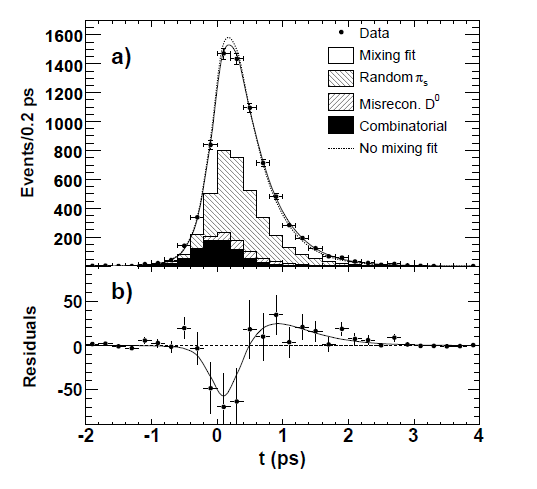
\includegraphics[scale=0.4]{figs/BaBar_D0_Mixing_Results.png}
\end{center}
\caption{\textit{ }}
\label{BaBar_D0_Mixing_Results.png}
\end{figure}
